\documentclass[12pt, a4paper]{article}
\usepackage{amsfonts, amsmath, amsthm}
\usepackage[utf8x]{inputenc}
\usepackage{indentfirst}
\usepackage{multirow}
\usepackage[table]{xcolor}
\usepackage{listings}
\usepackage{alltt}
\usepackage{fancyvrb}
\usepackage{amsmath}
\usepackage{graphicx}
\usepackage{algorithm}
\usepackage{algpseudocode}
\usepackage{subfigure}
\usepackage{setspace}
\usepackage{wrapfig}
\usepackage{colortbl}
\usepackage{wrapfig}
\usepackage{tikz}
\usetikzlibrary{positioning}

\graphicspath{ {./images/} }

\newtheorem{definitie}{Definitia}
\newtheorem{propozitie}{Propozitia}

\title{\bf Serenity Garden TD}
\author{Opria Ion-Bogdan}

\begin{document}
	\maketitle
	
	\tableofcontents
	\pagebreak
	
	\section{Introducere}
	
	\subsection{Descrierea proiectului}
	
	Jocurile video au inceput sa acapareze din ce in ce mai mult vietile noastre datorita usurintei de accesibilitate si a experientei pe care o ofera. Odata cu evolutia hardware-ului, jocurile video au devenit din ce in ce mai realiste si prin urmare ofera experiente care nu poat fi gasite in niciun alt mediu existent, deoarece in nici un alt mediu nu putem controla si traii experientele unor caractere atat de indetaliat. Industria jocurilor video este o industrie care este in continua crestere si prin urmare este o ramura care merita explorata din perspectiva unui programator si nu nu mai. 
	
	"Games are great to work on because they are as much about art as they are science." \cite{gameProgrammingComplete}
	
	Din aceste motive, am ales drept proiect pentru licenta sa fac un joc video. Jocul se numeste "Serenity Garden" si este un tower defense 3D. Experienta jocului are loc pe niste nivele special definite, in care utilizatorul trebuie sa isi proiejeze baza. Exista multe tipuri diferite de inamici care vor sa distruga baza player-ului, iar acesta, pentru a o proteja, trebuie sa construiasca un sistem defensiv pentru a ii tine la distanta. Player-ul poate sa construiasca turnuri defensive care au diferite efecte asupra inamicilor. Inamicii ataca tot ce gasesc in cale, iar daca reusesc sa distruga baza, player-ul pierde nivelul curent.
	
	Player-ul nu poate sa construiasca turnuri oriunde, ci are locuri predefinite unde poate sa le construiasca, locuri specificate de blocuri hexagonale pe mapa. Odata plasata o tureta, aceasta nu poate fi mutata, dar player-ul are si un caracter invulnerabil pe care il poate muta oriunde doreste pe mapa. Acest caracter va ataca inamicii automat cand nu se afla in miscare, si poate intra in turete pentru a le creste puterea/eficienta.
	
	Modul care va diferentia acest joc de celelalte jocuri pe acest stil este modul de co-op. 2 jucatori se vor putea conecta prin retea si vor juca un nivel dificil care necesita cooperare si o planificare buna intre ei.
	
	\subsection{Introducere in Game Development}
	
	\subsubsection{Scurta istorie}
	
	\subsubsection{Industria curenta}
	
	
	
	\section{Introducere in Unity}
	
	\subsection{Prezentare generala}
	
	
	\subsubsection{GameObject si Mesh}
	
	\subsubsection{Collider}
	
	\subsubsection{Transform si Rigidbody}
	
	\subsubsection{API-ul de scriptare}
	
	\subsection{Motivul alegerii pentru proiectul de licenta}

	\subsection{Elemente specifice folosite}	
	
	\subsubsection{Shader Graph}
	
	
	
	
	
	\section{Planificare Proiect}
	
	\subsection{Faza de Proiectare}
	
	"Almost anything that you can be good at can become a useful
	skill for a game designer." \cite{bookOfLenses}
	
	Din proiecte precedente am realizat ca o planificare buna a unui proiect inca de la inceput poate imbunatatii calitatea proiectului explonential, asigura usurinta de adaugare a unor elemente noi (fara sa fie necesara rescrierea/reorganizarea proiectului) si reduce frustrarea programatorilor care lucreaza la proiect.
	
	Din acest motiv, inca de la inceputul proiectului am incercat sa imi planific cat mai indetaliat continutul acestuia si modul in care il voi implementa.
	
	In prima faza, mi-am scris un design document care continea descrierea si elementele jocului, privite din multe perspective.
	
	Introducerea proiectului a fost realizata la inceputul acestui document si nu va fi reluata aici.
	
	
	
	\subsection{Tematica Jocului}
	
	Jocul are loc in viitorul departat. Planeta ta este supra-populata si nivelul de poluare a ajuns la un nivel critic. Umanitatea a trecut de mult de punctul in care mai pot salva aceasta planeta. Intreaga planeta va muri in cateva decenii, iar oamenii daca nu isi gasesc o alta casa intre timp, vor muri si ei cu ea. In acest scop, o armata speciala a fost formata, care are ca scop explorarea altor planete si gasirea unei planete care poate suporta rasa umana.
	
	Universul este totusi foarte periculos. Unele planete au viata extraterestra foarte agresiva, iar altele au fost distruse de experimente cibernetice esuate. Player-ul este comandantul suprem al acestei armate care are ca scop protejarea oamenilor de stiinta care vor analiza aceste planete.
	
	Prima faza a proiectului va contine o singura planeta care poate fi populata dar care contine multi inamici periculosi.
	
	Planeta mama trimite resurse din cand in cand, dar numai un numar limitat de resurse pot fi trimise deodata, iar acestea dureaza mult timp sa ajunga, asa ca nu putem depinde de ele in timpul unei lupte.
	
	
	
	\subsection{Caracterele Jocului}
	
	\textbf{Comandantul} este protagonistul jocului. El este caracterul din a carui perspectiva vom juca jocul. A fost cobaiul unui experiment menit sa creeze super-soldati, iar in urma acestui experiment a primit o putere speciala. Poate sa isi ascunda complet prezenta fata de alti oameni/alte creaturi. Din acest motiv, el este caracterul invulnerabil pe care il putem misca pe mapa in lupta.
	
	\textbf{Locotenentul} este este ajutorul tau numarul 1. El/ea iti va prezenta tutorialele, iti va da sfaturi si va juca un rol vital in poveste, in caz ca proiectul ajunge in acest punct.
	
	
	
	\subsubsection{Inamicii}
	\begin{itemize}
		\item \textbf{Melee} este un tip de inamic care poate ataca turetele doar cand sta fix in fata lor. Are viata mai multa decat inamicii "ranged".
		\item \textbf{Ranged} este un tip de inamic care poate ataca turetele de la distanta. Are viata putina, dar pot ataca repede.
		\item \textbf{Flying} este un inamic care poate fi lovit doar de un numar limitat de turete.
		\item \textbf{Ambusher} este un tip de inamic care ignora turnurile din cale. Acesta se misca pe cel mai scurt drum catre baza player-ului, iar daca ajunge deasupra acesteia, va lansa bombe care ii vor scadea drastic viata, dupa care vor pleca de pe mapa. Este un tip de inamic zburator care poate fi lovit doar de un numar limitat de turnuri.
	\end{itemize}

	Acesti inamici (cu exceptia ambusher-ului) se vor misca pe mapa calculand cel mai scurt drum catre baza player-ului. Daca acestia intalnesc in cale un turn, se vor opri si vor ataca acel turn. Cand turnul este distrus, ei isi vor relua drumul.
	
	Pentru fiecare inamic vor fi 3 tipuri de variatii, fiecare mai puternic decat cel precedent.
	
	
	
	\subsubsection{Turnuri defensive}
	In continuare voi scrie o descriere scurta pentru fiecare turn din joc. Toate proprietatile despre care urmeaza sa vorbesc sunt in comparatie cu celelalte turnuri defensive.
	\begin{itemize}
		\item \textbf{Serenity} este baza playerilor. Are viata foarte multa daca este distrusa player-ul pierde jocul si poate ataca inamicii care se apropie de ea. Are raza de atac medie, putere de atac medie, poate ataca orice tip de inamic si rata de reincarcare intre atacuri este mica (dureaza mult timp sa se reincarce)
		\item \textbf{Machine Gun} (fig: \ref{fig: machineGun}) este turnul pe care il primim la inceputul jocului. Are viata mica, poate ataca orice tip de inamic, are raza medie, damage mic si rata de atac este mare (araca foarte des)
		\item \textbf{Electric Fence} (fig: \ref{fig: electricFence}) este turnul de protectie. Are viata foarte mare, poate ataca doar inamicii "melee", damage-ul este mediu si rata de reincarcare este mica. Scopul acestui turn este sa stea in calea inamicilor pentru a fi atacat de inamici, iar in timpul acela, celelalte turete pot distruge inamicii.
		\item \textbf{Vulkan} (fig: \ref{fig: vulkan}) Este tureta speciala impotriva inamicilor zburatori. Are damage mult dar poate ataca doar inamici zburatori, viata putina si raza de atac mare.
		\item \textbf{Machine Cannon} (fig: \ref{fig: machineCannon}) este un turn care este foarte puternic impotriva inamicilor "melee". Are damage mare, rata de atac mica, viata medie, raza mica si prioritizeaza inamicii melee pe cat posibil.
		\item \textbf{Railgun} (fig: \ref{fig: railgun}) este un turn care este foarte puternic impotriva inamicilor "ranged". Are damage mare, rata de atac mica, viata medie, raza mica si prioritizeaza inamicii ranged pe cat posibil.
		\item \textbf{Excavator} (fig: \ref{fig: excavator}) este un tip special de turn deoarece nu poate ataca inamicii. Acesta aduna resurse in timpul luptei, resurse care pot fi convertite in bani de joc. Are viata multa, si pentru ca nu poate ataca, trebuie aparat de inamici.
	\end{itemize}
	
	
	\begin{figure}[H]
		\centering
		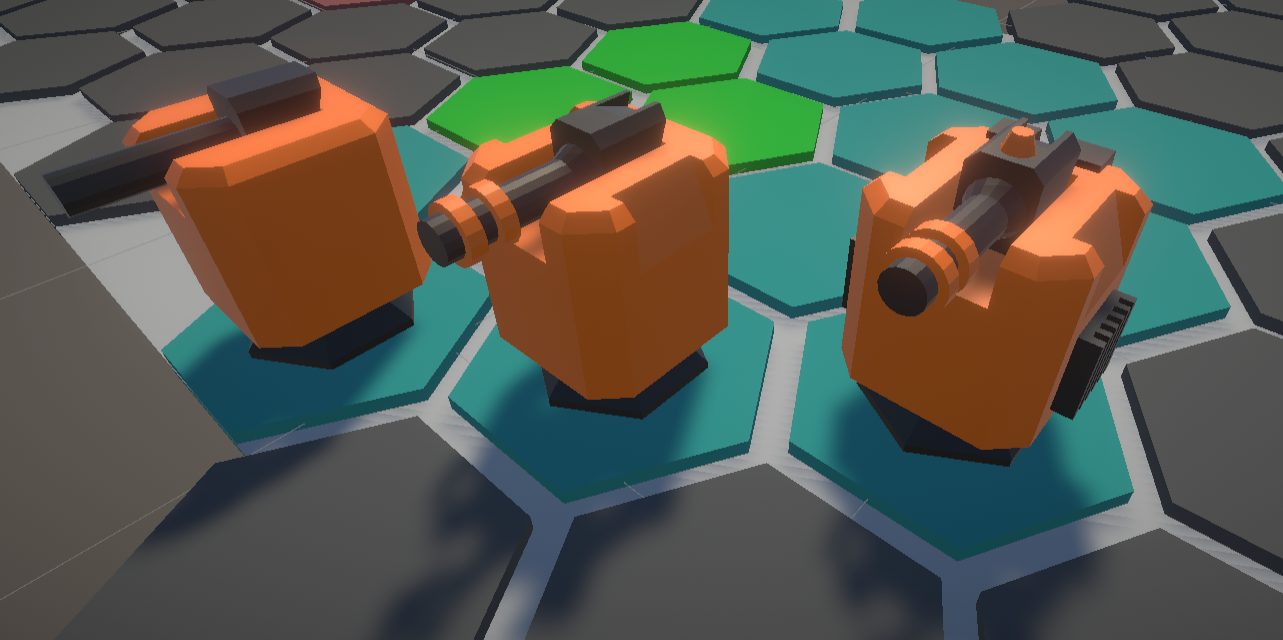
\includegraphics[width=1\textwidth]{machineGun.png}
		\caption{Machine Gun}
		\label{fig: machineGun}
	\end{figure}

	\begin{figure}[H]
		\centering
		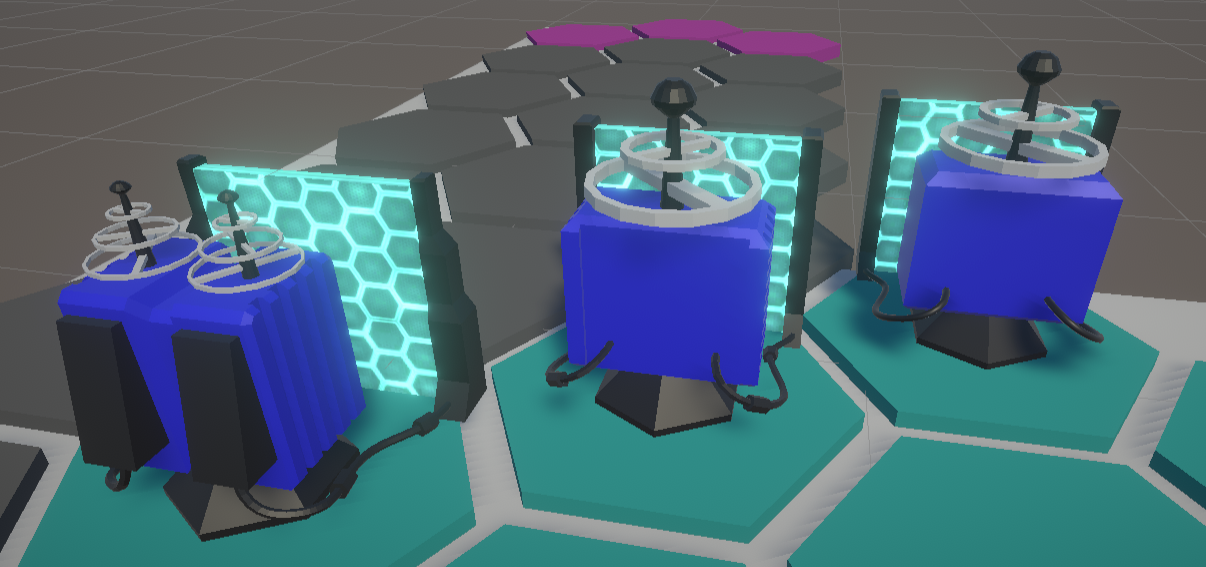
\includegraphics[width=1\textwidth]{electricFence.png}
		\caption{Electric Fence}
		\label{fig: electricFence}
	\end{figure}

	\begin{figure}[H]
		\centering
		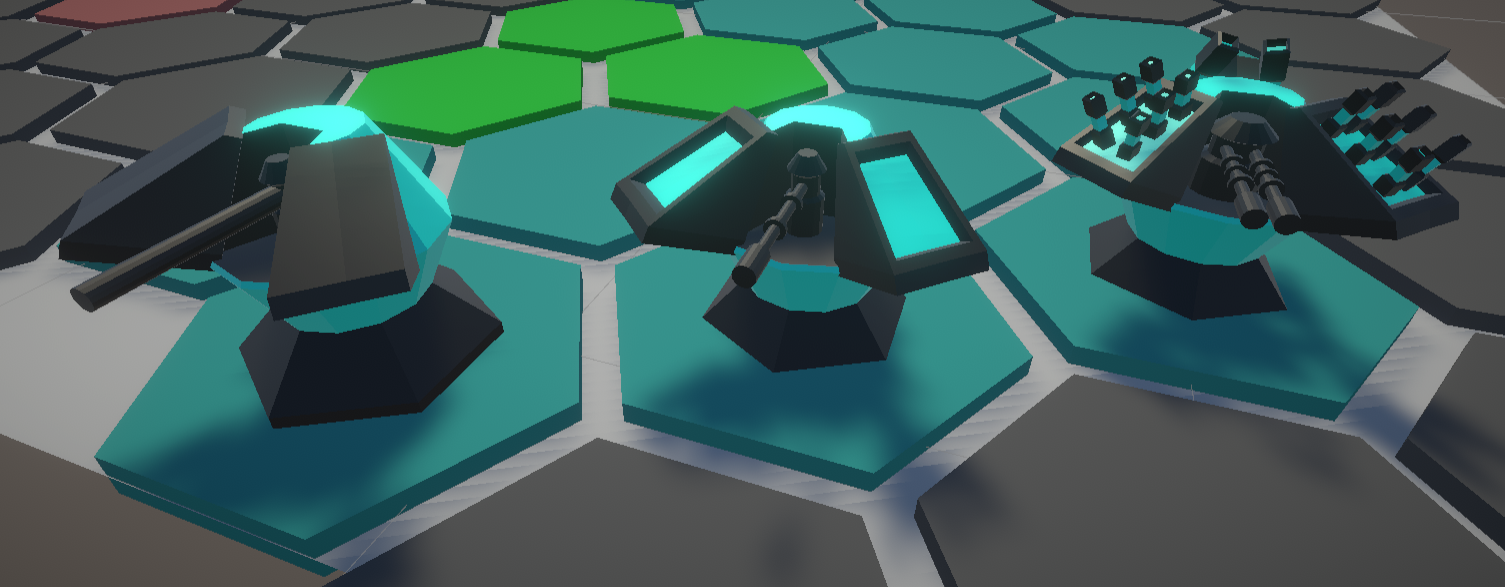
\includegraphics[width=1\textwidth]{vulkan.png}
		\caption{Vulkan}
		\label{fig: vulkan}
	\end{figure}

	\begin{figure}[H]
		\centering
		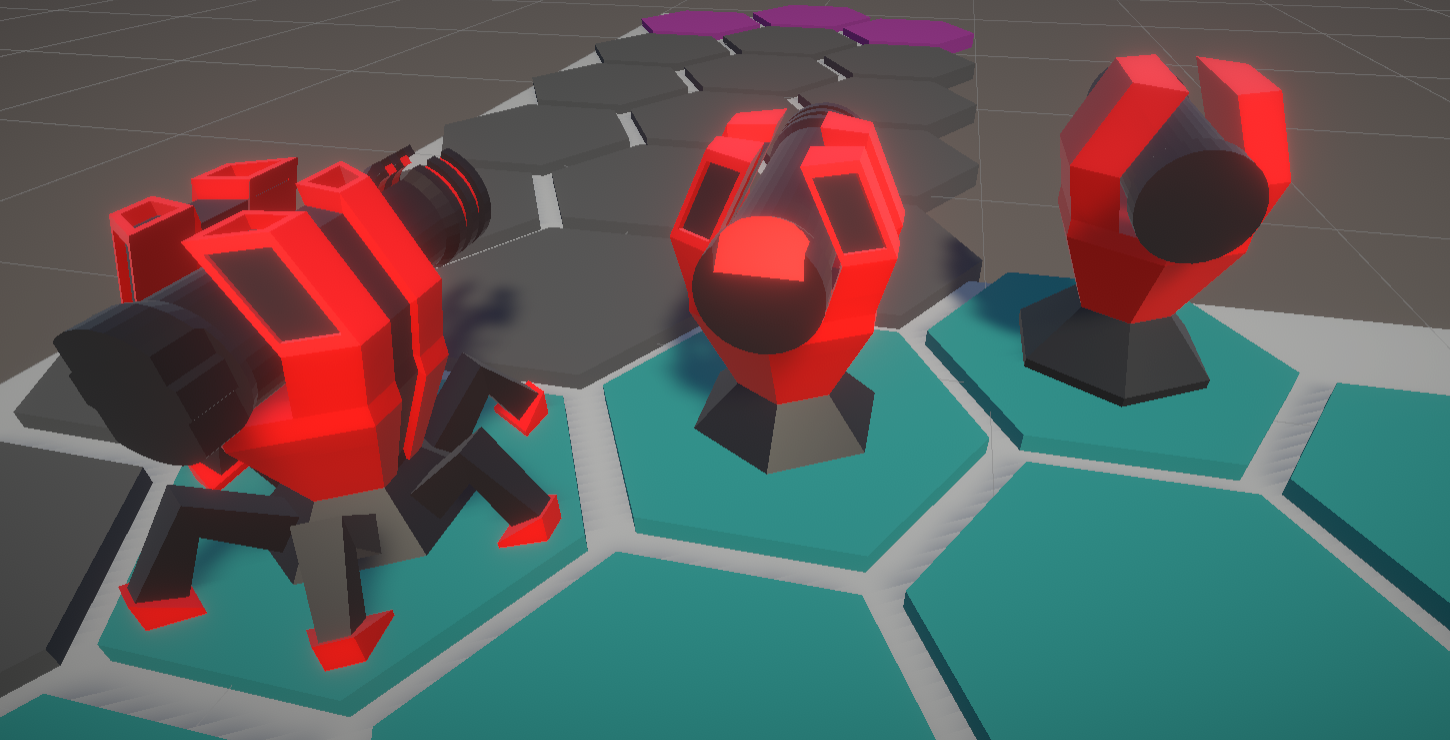
\includegraphics[width=1\textwidth]{machineCannon.png}
		\caption{Machine Cannon}
		\label{fig: machineCannon}
	\end{figure}
	
	\begin{figure}[H]
		\centering
		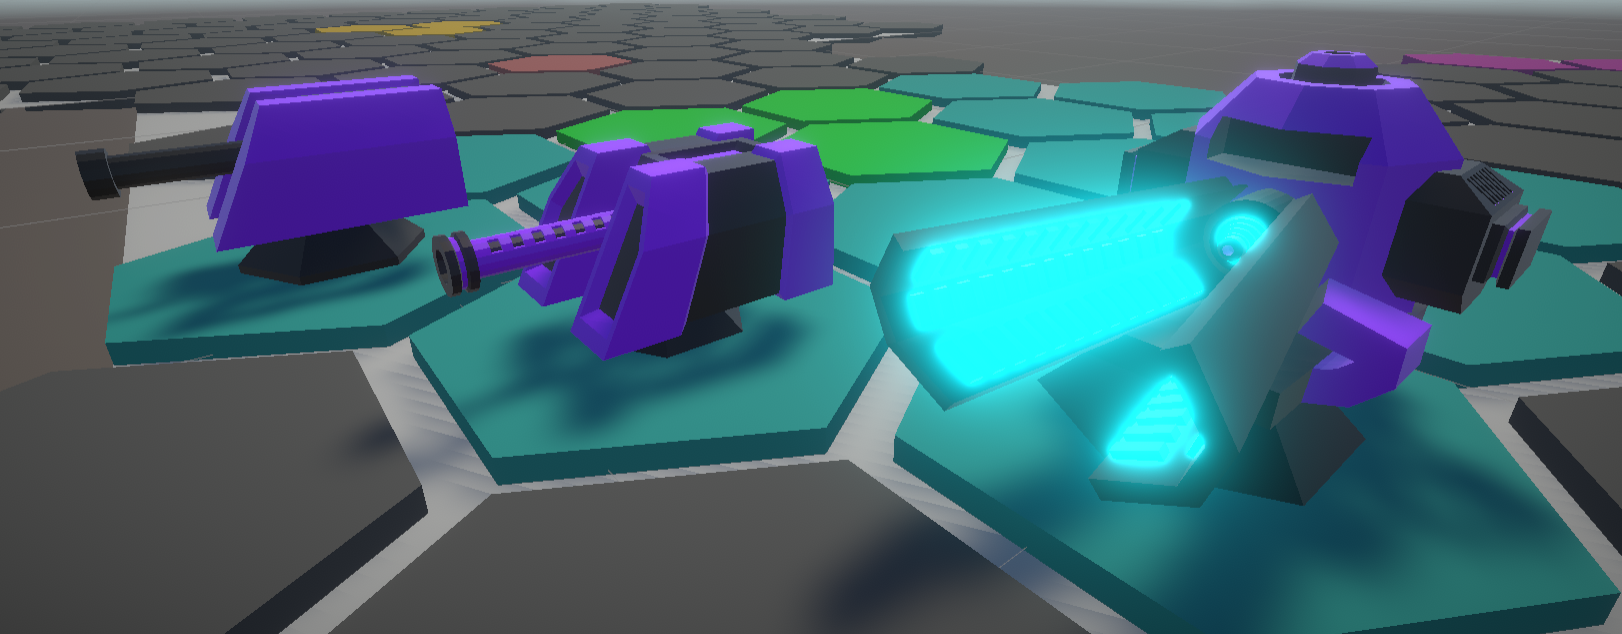
\includegraphics[width=1\textwidth]{railgun.png}
		\caption{Railgun}
		\label{fig: railgun}
	\end{figure}

	\begin{figure}[H]
		\centering
		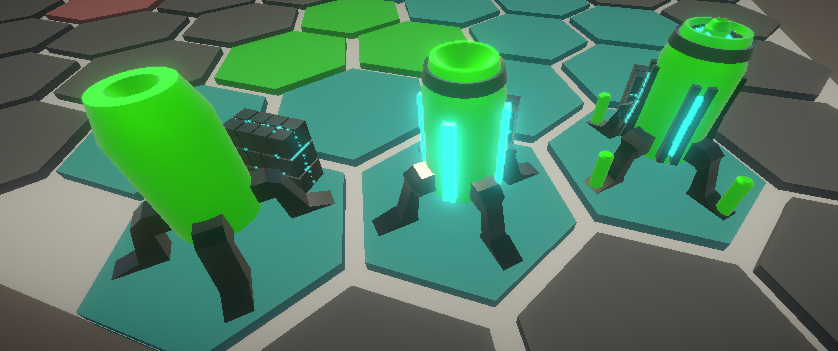
\includegraphics[width=1\textwidth]{excavator.png}
		\caption{Excavator}
		\label{fig: excavator}
	\end{figure}
	
	
	
	\subsection{Sistemele Jocului}
	
	\subsubsection{Mapa}
	
	Pe mapa jocului vor fi generate automat obiecte hexagonale. Aceste obiecte pot fi de mai multe tipuri:
	\begin{itemize}
		\item Hexagoane goale (cele gri din (fig: \ref{fig: gridSystem})).
		\item Hexagoane pe care putem construii turnuri de atac. (cele albastre din (fig: \ref{fig: gridSystem}))
		\item Hexagoane pe care putem construii turnul de extragere de resurse. (cele verzi din (fig: \ref{fig: gridSystem}))
		\item Hexagonul pe care va incepe si se va afla comandantul. Cand acesta se misca, locul in care se misca va deveni si el un astfel de hexagon. (cel roz din (fig: \ref{fig: gridSystem}))
		\item Hexagoanele bazei. Baza va ocupa 3 hexagoane de acest tip. (cele galbene din (fig: \ref{fig: gridSystem}))
		\item Hexagonul ocupat. Fiecare hexagon care este ocupat de o anumita structura devine un astfel de hexagon. (va avea culoarea rosie)
	\end{itemize}

	Inamicii isi vor calcula drumul pe care merg in functie de toate aceste tipuri de hexagoane. Din acest motiv este nevoie si de cel gol.
	
	\begin{figure}[H]
		\centering
		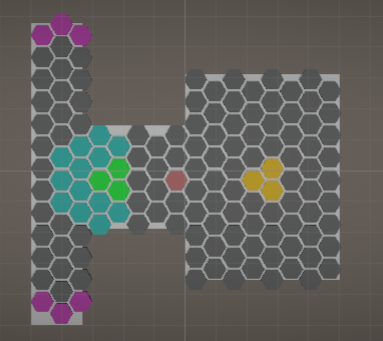
\includegraphics[width=1\textwidth]{grid.png}
		\caption{Hexagonal Grid}
		\label{fig: gridSystem}
	\end{figure}


	
	\subsubsection{Sistemul Turnurilor}
	
	Turnurile pot fi plasate doar pe hexagoanele de constructie. Odata plasate, acestea nu pot fi mutate. Singurele metode de a goli acel hexagon este sa fie distrus de un inamic sau sa vindem tureta. Daca vindem o tureta, vom primi inapoi o parte din banii investiti. Acestea pot fi upgradate, dar acest sistem va fi deblocat la anumite stagii din joc. Toate turnurile au urmatoarele proprietati:
	\begin{itemize}
		\item Attack Speed
		\item Damage
		\item Health
		\item Range
		\item Attack type (specifica ce tip de inamici putem sa atacam)
	\end{itemize}

	Daca viata turetei ajunge la 0, va fi distrusa automat. Atata timp cat o tureta nu este distrusa, o putem repara, dar reparatiile vor fi executate intr-un anumit timp, iar in acest timp, tureta nu va putea sa atace.
	
	\subsubsection{Comandantul}
	
	Comandantul poate fi mutat pe orice hexagon care nu este deja ocupat. Dupa ce ai ales un hexagon, acesta va incepe sa se miste catre acesta. Cat timp este in miscare, nu poate ataca inamicii. Destinatia poate fi schimbata doar dupa ce a ajuns la destinatie. Are raza medie, rata de atac medie, damage mediu si poate ataca orice tip de inamic.
	
	Acesta poate intra si in turete, imbunatatindu-le status-urile.
	
	\subsubsection{Tura de lupta (enemy wave)}
	
	Jocul va avea mai multe nivele, care pot fi selectate dintr-un meniu. Nivelele vor fi cat mai diferite posibil. Inamicii au mai multe puncte din care pot sa vina in functie de nivelul ales. Acestia vin in grupuri de inamici. Intre fiecare grup exista o perioada de repaus in care player-ul isi poate repara turnurile. In caz ca nu are nevoie de reparari, poate selecta sa sara peste perioada de repaus, astfel primind bani extra.
	
	
	
	\subsubsection{Nivelele jocului}
	
	Nivelul este terminat cand toti inamicii au fost omorati. Fiecare nivel va avea un scor de maxim 3 stele, care specifica cat de bine ne-am descurcat la acest nivel. Scorul este calculat in functie de mai multe proprietati, precum, viata ramasa a bazei la final, numarul de inamici omorati, numarul de turete ramase in viata (daca construim 12 si pierdem 2, acest scor nu va fi maxim). Fiecare stea castigata va da bani extra, bani care pot fi folositi in magazinul de upgrade-uri permanente, despre care vom discuta in scurt timp.
	
	Playerul poate sa joace din nou nivelele, dar nu va mai primii atat de multi bani ca prima data. Acesta va castiga bani extra de pe stelele castigate doar daca a primit mai multe stele decat turele anterioare.
	
	
	
	\subsubsection{Lock-on}
	
	Jucatorul poate sa apese pe inamici, astfel setand acel inamic drept o prioritate. Fiecare turn care poate ataca acest tip de inamic il va prioritiza fata de alti inamici. De indata ce este omorat, se pierde aceastra prioritate.
	
	
	
	\subsubsection{Magazinul de upgrade-uri permanente}
	
	Intre nivele putem sa cumparat piese de schimb pentru turnurile noastre pentru a le face mai puternice. Aceste piese se pot cumpara doar cu banii castigati de pe urma nivelelor. Upgrade-urile in functie de turn sunt urmatoarele:
	
	\begin{itemize}
		\item Machine gun: atac mai puternic, range mai mare, costuri mai mici.
		\item Electric fence: mai multa viata, atac mai puternic, costuri mai mici.
		\item Vulkan: atac mai puternic, range mai mare, atac mai rapid
		\item Machine cannon: atac mai puternic, range mai mare, atac mai rapid
		\item Railgun: atac mai puternic, range mai mare, atac mai rapid
		\item Excavator: da bani mai multi, timpul intre livrarile de bani mai scurt, cumpara upgrade-uri.
	\end{itemize}
	
	Fiecare upgrade va avea mai multe nivele, fiecare costand din ce in ce mai multi bani, dar vor avea un nivel maxim la care putem duce upgrade-urile.
	
	
	
	\subsubsection{Raid system}
	
	Cand un jucator alege acest mod, va putea sa aleaga din o serie de mape. Fiecare mapa are un monstru foarte puternic pe care trebuie sa il bata impreuna cu un alt jucator. Dupa ce a selectat mapa, va fi trimis la un ecran de asteptare, in care va sta pana cand se va gasi un alt jucator care a selectat acea mapa. Dupa ce a fost gasit un coechipier, vor incepe jocul. Undeva pe mapa se va afla un monstru imens si ei trebuie sa isi protejeze baza de acest monstru. Momentan tipurile de monstrii la care m-am gandit sunt urmatoarele:
	
	\begin{itemize}
		\item \textbf{Fire Demon} este un monstru din lava care din cand in cand loveste turetele si baza, provocand o tona de daune. Monstrul trebuie omorat cat de repede posibil ca sa nu distruga baza inainte.
		\item \textbf{Necromancer} este un monstru care cheama alti monstrii pe mapa. Puterea lui sta in spatele intregii armate ale lui. Daca playerii sunt complesiti de aceasta armata vor pierde nivelul. Trebuie sa aiba un echilibru bun intre defensiva si ofensiva.
		\item \textbf{Armadillo} este un care ataca periodic baza. Da mai putin damage decat "Fire Demon", dar are si un tip de atac in care se face ghem si incepe sa se roteasca. Daca playerii nu ii dau suficient de mult damage in timpul ala sau nu fac anumite actiuni specifice (ex: sa mute comandantul intr-un anumit loc sau sa construiasca o tona de turete in calea lui), el va ataca baza, dand foarte mult damage.
	\end{itemize}

	Fiecare player poate plasa turete oriunde. Playerii pot plasa turete unul peste tureta celuilalt, astfel activand un efect special. Acestia pot sa isi upgradeze doar turetele construite de ei. Amandoi playerii au caracterele lor comandant, dar acestia nu pot intra in aceeasi tureta in acelasi timp. Pentru sistemul de lock-on, doar turetele player-ului care a setat lock-on-ul va ataca inamicul prioritizat.
	
	
	\subsection{Analiza proiectului din punctul de vedere al consumatorilor}
	
	\subsubsection{Dificultatea jocului}
	
	Jocul va fi relativ dificil. Trebuie sa te gandesti unde sa construiesti anumite turete pentru a folosi resursele cat mai bine. La inceput jocul va fi usor, dar pe urma va trebui sa te gandesti foarte bine unde sa plasezi anumite turete, altfel vei pierde nivelul. Trebuie sa se gandesti si daca poti rezista sa sari peste perioada de repaus intre grupurile de inamici.
	
	Sistemul de raid are un nivel de dificultate cu mult mai ridicat, pentru ca trebuie sa te si coordonezi cu un alt jucator.
	
	
	
	\subsubsection{Elemente de dependenta}
	
	In caz ca nu putem depasii un anumit nivel, putem juca nivelele anterioare si sa ne asiguram ca luam 3 stele la fiecare nivel. Aceasta metoda de a obtine 3 stele la fiecare nivel poate fi unul din motivele care ii determina pe jucatori sa continue sa joace jocul. Un alt factor ar putea fi sistemul de upgrade-uri permanente.
	
	
	
	\subsubsection{Grupele de varsta vizate}
	
	Acest joc nu are limitari de varsta, poate fi jucat de oricine, dar va fi apreciat cel mai mult de copii si de adolescentii care cauta provocari in jocurile de strategie. Jocul este in principiu facut pentru "casual gamers".
	
	
	
	\section{Implementare proiect}
	
	\subsection{Scena de lupta}
	
	\subsubsection{Initializarea scripturilor}
	
	In unity scripturile au cateva metode care ajuta la initializare.
	
	\textbf{Awake} este metoda care este apelata la inceputul programului si inainte de restul metodelor.
	
	\textbf{Start} este metoda care este apelata dupa ce s-au apelat metodele Awake de la toate scripturile.
	
	\textbf{Update} este apelat la fiecare frame al jocului, aici intervine o mare parte din logica jocurilor. Apelarea update-ului incepe dupa ce toate metodele "Start" au fost apelate.
	
	Pentru "Start" si "Awake", unity decide automat in ce ordine sa le apeleze, fara ca noi sa putem controla acest lucru. In multe proiecte mai complexe se ajunge in momentul cand pentru initializatea anumitor sisteme este necesar ca alte sisteme sa fie deja initializate. Cum nu putem controla ordinea de initializare, se ajunge in punctul in care putem primi erori random din cauza initializarii haotice.
	
	Pentru a combate asta, m-am gandit la un sistem care va permite controlarea initializarii tuturor procese cu usurinta.
	
	\begin{figure}[H]
		\centering
		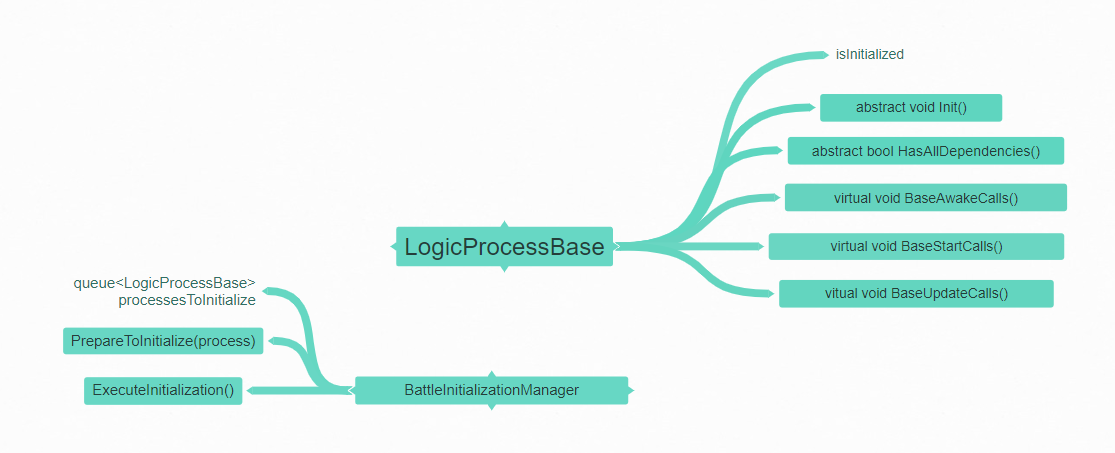
\includegraphics[width=1\textwidth]{logicProcessCoggle.png}
		\caption{Initializarea scripturilor}
		\label{fig: logicProcessCoggle}
	\end{figure}
	
	Am creat clasa LogicProcessBase, pe care, toate scripturile care au nevoie de o initializare mai organizata, trebuie sa o mosteneasca si care contine:
	\begin{itemize}
		\item \textbf{isInitialized} care specifica daca scriptul curent a fost initializat sau nu inca
		\item \textbf{Init()}. In aceasta metoda trebuie sa scriem tot codul de initializare a clasei care mosteneste.
		\item \textbf{HasAllDependencied()}. Este o metoda care returneaza un boolean. In aceasta clasa trebuie sa punem toate dependintele de care are nevoie clasa care mosteneste.
		\item \textbf{BaseAwakeCalls()}. In aceasta metoda apelam "PrepareToInitialize()" din clasa "BattleInitializationManager", despre care vom vorbi in scurt timp.
		\item \textbf{BaseStartCalls()} si \textbf{BaseUpdateCalls()} sunt metode in care trebuie sa scriem tot codul care normal ar fi venit in Start/Update. In unity, nu putem defini Start/Update drept virtual si sa modificam functiile lor pe urma, din acest motiv tot codul din clasele dintr-o ierarhie mai complexa trebuie sa fie scris in aceste metode, iar in clasa cel mai jos din ierarhie trebuie sa le apelam in Awake/Start/Update.
	\end{itemize}

	\textbf{BattleInitializationManager} este a doua clasa de care avem nevoie. Ea este responsabila pentru a executa initializarea propriuzisa a proceselor. 
	
	\textbf{PrepareToInitialize()} este apelata de fiecare proces in metoda lor de awake, iar aceasta metoda va adauga procesul intr-o coada.
	
	\textbf{ExecuteInitialization()} parcurge toate procesele din coada si verifica daca acestea pot fi initializate, apeland "HasAllDependencies()". Daca procesul curent poate fi initializat, atunci ii apeleaza metoda "Init()" si seteaza "isInitialized = true". Daca nu il poate initializa, il adauga la finalul cozii pentru a fi initializat la final. Acest proces se repeta pana cand coada este goala sau s-a parcurs o data coada cap-coada si nu s-a initializat nici un proces. In acest caz inseamna ca aveau dependinte circulare si oprim procesul de initializare, afisand un mesaj de eroare. Aceasta metoda trebuie apelata in Awake, Start si Update, deoarece, pe parcurs pot aparea noi procese care trebuie initializate, iar programul trebuie sa poata sa detecteze astfel de cazuri.
	
	\subsubsection{Procesarea comenzilor venite de la utilizator}
	
	\subsubsection{Grid system}
	
	\subsubsection{Sistemul de navigare}
	
	Caracterele jocului trebuie sa stie pe unde pot sa mearga ca sa ajunga la o anumita destinatie. In acest scop a trebuit sa aleg un algoritm care sa imi gaseasca cel mai scurt drum posibil. Dupa o investigare amanuntita am ales sa folosesc algoritmul Floyd-Warshall.
	
	"Consideram reteaua orientata $G = (N, A, b)$ reprezentata prin matricea valoare adiacenta $B = (b_{ij}), i, j \in N$ cu
	
	\begin{equation*}
		b_{ij} = \begin{cases}
			b(i, j) \quad daca \quad i \neq j \quad si \quad (i, j) \in A; \\
			0 \quad daca \quad i = j; \\
			\infty \quad daca \quad i \neq j \quad si \quad (i, j) \neq A.
		\end{cases}
	\end{equation*}

	Algoritmul Floyd-Warshall determina matricea distantelor $D = (d_{ij}), i, j \in N$ si matricea predecesor $P = (p_{ij}), i, j \in N$." \cite{grafuriAnul2}
	
	\begin{algorithmic}
		\Function{Floyd-Warshall}{}
			\For{i $\gets$ 1 to n}
				\For{j $\gets$ 1 to n}
					\State $d_{ij} \gets b_{ij};$
					\If{i $\neq$ j and $d_{ij} < \infty$}
						\State $p_{ij} = i;$
					\Else
						\State $p_{ij} = 0;$
					\EndIf
				\EndFor
			\EndFor
			
			\For{k $\gets$ 1 to n}
				\For{i $\gets$ 1 to n}
					\For{j $\gets$ 1 to n}
						\If{$d_{ik} + d_{kj} < d_{ij}$}
							\State $d_{ij} = d_{ik} + d_{kj};$
							\State $p_{ij} = p_{kj};$
						\EndIf
					\EndFor
				\EndFor
			\EndFor
		\EndFunction
	\end{algorithmic}

	\begin{algorithmic}
		\Function{Reconstruire Drum}{}
			\State k = n;
			\State $x_k = j$
			\While{$x_k \neq i$}
				\State $x_{k - 1} = p_{ix_k};$
				\State k = k - 1
			\EndWhile
		\EndFunction
	\end{algorithmic}

	Drumul minim este $D_{ijp} = (x_k, x_{k+1}, \dots, x_{n-1}, x_n) = (i, x_{k+1}, \dots, x_{n-1}, j)$
	
	O alternativa pe care am considerat-o pentru algoritmul de navigare a fost algoritmul lui Dijkstra. Acesta este de asemenea un algoritm care gaseste cel mai scurt drum intre 2 noduri si se bazeaza pe relatiile urmatoare:
	\\
	
	$d(s, x_h) = \sum_{i=1}^{h} b(x_{i-1}, x_i)$.
	
	$d(x_{j+1}) \leq d(x_j) + b(x_j, x_{j+1}) = d(s, x_j) + b(x_j, x_{j+1}) = d(s, x_{j+1}) \leq d(s, z)$.
	
	$d(y) = min\{d'(y), min\{d'(x) + b(x, y) | x \in V^-(y)\}\}$.
	\\
	
	In cele din urma am ales Floyd-Warshall, deoarece, chiar daca are complexitatea mai mare, va fi rulat o singura data in tot programul, iar reconstruirea drumului se intampla aproape instantaneu. Mapa nu se va schimba pe parcursul jocului, iar din acest motiv am considerat ca e o optiune mai buna decat alti algoritmi precum Dijkstra sau A*.
	
	\subsubsection{Ierarhia inamicilor}
	
	\subsubsection{Ierarhia turnurilor defensive}
	
	
	\subsection{Selectarea nivelelor}
	
	
	
	\subsection{Magazinul de upgrade-uri permanente}
	
	
	
	\subsection{Sistemul co-op}
	
	
	
	
	\section{Concluzii}
	
	
	\pagebreak
	\begin{thebibliography}{3}
		\bibitem{gameProgrammingComplete} 
		Mike McShaffry, David Graham. \newline
		\textit{Game Coding Complete Fourth Edition}. 2012
		
		\bibitem{bookOfLenses}
		Jesse Schell.  \newline
		\textit{The Art of Game Design: A Book of Lenses 1st Edition}. 2008
		
		\bibitem{grafuriAnul2}
		Eleonor Ciurea, Laura Ciupala.  \newline
		\textit{Algoritmi: Introducere in algoritmica fluxurilor in retele}. 2006
		
	\end{thebibliography}
	
	
\end{document}